\documentclass[9pt,lineno,doublespacing]{elife}
% \documentclass[9pt,lineno,]{elife}
\usepackage{nameref}
\usepackage{tikz}
\usetikzlibrary{arrows,shapes,arrows.meta}
\usepackage{setspace}
\usepackage{booktabs}
\usepackage{colortbl}
\usepackage{mathtools}
\usepackage{siunitx}
\usepackage{tabularx}
\usepackage{sidecap}
\usepackage{wrapfig}

% glossaries. Disable the link in main document.
\usepackage[acronym]{glossaries}
\loadglsentries{glossaries}
\usepackage{siunitx}
\DeclareSIUnit\Molar{M}
\glsdisablehyper

\title{Subunit exchange enhances information retention by CaMKII in dendritic spines}

\author[]{Dilawar Singh}
\author[]{Upinder Singh Bhalla}

\affil[]{National Centre for Biological Sciences Bangalore, Tata Institute of Fundamental Research}
\corr{bhalla@ncbs.res.in}{USB}

\presentadd[]{National Centre of Biological Sciences Bangalore
    , Tata Institute of Fundamental Research, India
}

% macros for superscript and subscript.
\newcommand\SUB[2]{#1\textsubscript{#2}}
\newcommand\SUP[2]{#1\textsuperscript{#2}}
% \rowcolors{1}{gray!20}{white}

\begin{document}
\maketitle

% ABSTRACT
\begin{abstract}\label{abstract} 
Molecular bistables are strong candidates for long-term information storage, for
example, in synaptic plasticity. Calcium/calmodulin dependent protein Kinase II
(CaMKII) is a highly expressed synaptic protein which has been proposed to form
a molecular bistable switch capable of maintaining its state for years despite
protein turnover and stochastic noise. It has recently been shown that CaMKII
holoenzymes exchange subunits among themselves. Here we used computational
methods to analyze the effect of subunit exchange on the CaMKII pathway in the
presence of diffusion in two different micro-environments, the Post Synaptic
Density (PSD) and spine cytosol. CaMKII exhibits multiple timescales of activity
and subunit exchange enhances the information retention ability of CaMKII by
improving the stability of its switching in the PSD, and by slowing the decay of
its activity in the spine cytosol. The existence of diverse timescales in the
synapse has important theoretical implications for memory storage in networks.
\end{abstract}



\section{Introduction}\label{introduction}

Memories are believed to be stored in synapses, encoded as changes in synaptic
strength \citep{hebb_organization_2005,takeuchi_synaptic_2014,choi_interregional_2018}.
\gls{ltp}, an activity dependent change in synaptic strength, is considered to
be the primary post-synaptic memory mechanism
\citep{bliss_expression_2013,mayford_synapses_2012}. Various behavioural
experiments strongly suggest a critical role for \gls{camkii} in induction of
\gls{ltp} \citep{lucchesi_novel_2011,giese_autophosphorylation_1998}. In
the CA1 region of Hippocampus, blocking \gls{camkii} activity blocks the
induction of \gls{ltp} \citep{chang_camkii_2017}.  After LTP induction, several
other pathways including protein synthesis \citep{aslam_translational_2009},
clustering of receptors \citep{shouval_clusters_2005}, receptor translocation
\citep{hayer_molecular_2005} and PKM-$\zeta$ activation
\citep{sacktor_memory_2012}, have been suggested as mechanisms for long-term
maintenance of synaptic state. Recent evidence from behavioural assays suggests
that \gls{camkii} may also be involved in long-term maintenance of memory
\citep{rossetti_memory_2017} (but see \citep{chang_camkii_2017}).

Any putative molecular mechanism involved in long-term maintenance of memory
must be able to maintain its state despite the potent resetting mechanisms of
chemical noise and protein turnover.  In the small volume of the synapse ($\sim$
0.02 \si{\micro\meter^3} \citep{bartol_nanoconnectomic_2015}), the number of
molecules involved in biochemical processes range from single digits to a few
hundred, thereby increasing the effect of chemical noise.  Lisman proposed that
a kinase and its phosphatase could form a bistable molecular switch able to
maintain its state for a very long time despite turnover
\citep{lisman_mechanism_1985}. It has been shown by various mathematical models
that \gls{camkii} and its phosphatase \gls{pp1} may form a bistable switch
\citep{sandstorm_models_2004,zhabotinsky_bistability_2000} which can retain its
state for years despite stochastic chemical noise and protein turnover
\citep{miller_stability_2005}. Although there is experimental evidence that
CaMKII/PP1 is bistable in \emph{in vitro} settings
\citep{bradshaw_ultrasensitive_2003,urakubo_vitro_2014}, experimental evidence
for \emph{in vivo} bistability is lacking. In spine cytosol, \gls{camkii} has
been shown not to act like a bistable switch but rather a leaky integrator of
calcium activity \citep{chang_camkii_2017}.  However, \gls{camkii} may be
bistable in special micro-environments such as the ``core'' \gls{psd} where it
attaches to NMDA receptor \citep{dosemeci_postsynaptic_2016,
petersen_distribution_2003}.

From computational perspective, the CaMKII/PP1 bistable system is an attractive
candidate for memory storage \citep{koch_biophysics_2004}.  Bistability provides
a plausible solution to the problem of state maintenance. Previous modeling work
has shown that CaMKII/PP1 system may form a very stable switch despite protein
turnover and stochastic noise in the small volume of the synapse.  The stability
increases exponentially with the number of holoenzymes
\citep{miller_stability_2005}. It is important to note that this model exhibits
bistable behaviour only in a narrow range of \gls{pp1} concentrations in the
\gls{psd}. This strict restriction may be met because phosphorylated
\gls{camkii} is protected from phosphatases in \gls{psd} except \gls{pp1}
\citep{strack_differential_1997} which is tightly regulated in the \gls{psd}
\citep{bollen_extended_2010}. 

\gls{camkii} has another remarkable property which was hypothesized by Lisman
\citep{lisman_cam_1994} but discovered only recently, namely, subunit exchange.
In this process, two \gls{camkii} holoenzymes can exchange active subunits
leading to spread of \gls{camkii} activation \citep{stratton_activation-triggered_2014}.

In this paper, we adapt the model of \gls{mz} \citep{miller_stability_2005} to
include subunit exchange and diffusion, and quantify the effects of subunit
exchange on the properties of the CaMKII-PP1 system in two adjacent neuronal
micro-environments: \gls{psd} and spine cytosol. 

In the \gls{psd}, \gls{pp1} is tightly regulated and \gls{camkii} is protected
from other phosphatases. In the spine cytosol, \gls{camkii} is accessible to other
phosphatases along with \gls{pp1}. We examined how state switching lifetimes in
the \gls{psd} are affected by subunit exchange in different contexts of
\gls{pp1} levels, turnover, and clustering of \gls{camkii}. In the spine cytosol
we show how the integration of calcium stimuli generates two time-courses of
\gls{camkii} activity as a result of subunit exchange \citep{chang_camkii_2017}.

% RESULTS
\section{Results}\label{sec:results} 
\subsection{Model validation}\label{subsec:model-validation}

The basic computational units in our model are individual \gls{camkii} subunits
and \gls{camkii} ring consisting of 6 or 7 \gls{camkii} subunits. We treat the
\gls{camkii} ring as a proxy for the \gls{camkii} holoenzyme, which consists of
two such rings stacked over each other
\citep{woodgett_calmodulin-dependent,hoelz_crystal_2003}. In our model,
\gls{camkii} exists in 15 possible states compared to 2 in
\citep{miller_stability_2005} (see \nameref{sec:materials_and_methods}). This
leads to many more reactions than the \gls{mz} model. Since analytical
comparison of the two models was not possible, we first compared numerical
results from our model without diffusion and without subunit exchange with the
\gls{mz} model (\FIG{validation}).

\begin{figure}[t]%[hbt] 
    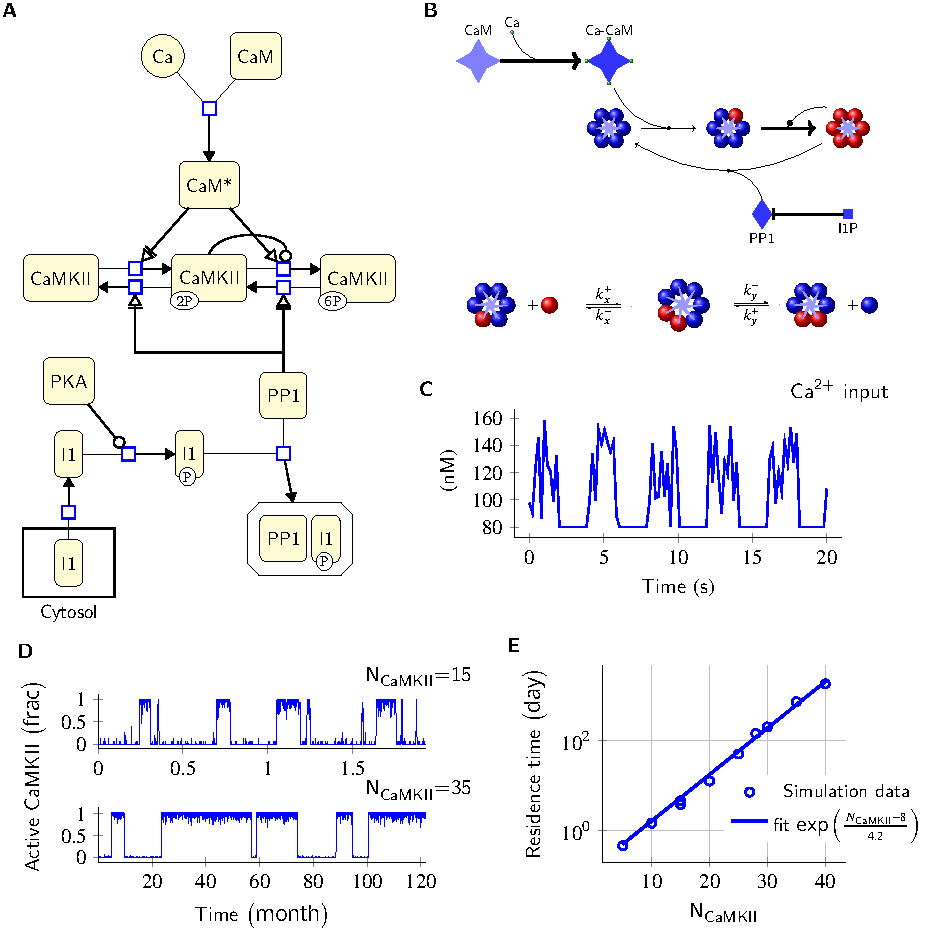
\includegraphics[width=0.95\linewidth]{./PaperFigures/elifeFigure1/figure_validation_178mm.pdf}
    \caption{Model description and validation. \textbf{(A)} CaMKII/PP1
        pathway described in \gls{sbgn} - Process Description (PD) Language \citep{novere_systems_2009}. 
        \textbf{(B)} \textbf{(above)} Major chemical reactions in the CaMKII/PP1 pathway. 
        \textbf{(below)} Subunit exchange between two \gls{camkii} holoenzymes. Red
        and blue balls represent phosphorylated and un-phosphorylated subunits
        respectively.  \textbf{(C)} Basal \gls{ca} profile in spine and
        \gls{psd} in all simulations. Basal \gls{ca} level is \SI{80}{\nano M} with fluctuations
        every \SI{2}{\second}, lasting for \SI{2}{\second}. These fluctuations are sampled from a uniform
        distribution with mean $\mu$ =\SI{120}{\nano M} and
        standard deviation of $\sigma$=\SI{23}{\nano M}.
        \textbf{(D)} Without diffusion and subunit exchange, CaMKII in our model is bistable.
        Two trajectories of \gls{camkii} activity (fraction of total \gls{camkii}
        holoenzymes with at least 2 subunits phosphorylated) are shown for different system
        size \SUB{N}{CaMKII}=15 (\textbf{top}) and \SUB{N}{CaMKII}=35 (\textbf{bottom}).
        \textbf{(D)} Switch stability increases exponentially with system size \SUB{N}{CaMKII}. The 
        average residence time of  switch's stable states increases exponentially
        with number of \gls{camkii} holoenzymes (\SUB{N}{CaMKII}). Turnover
        rate \SUB{v}{t}=\SI{30}{\per \hour}. Panels \textbf{(C, D, E)} show key
        properties of our model that are very similar to those of the \gls{mz} 
        model.}\label{fig:validation} 
    \figdata{Source and data is available at
    \url{http://github.com/dilawar/SinghAndBhalla_CaMKII_SubunitExchange_2018/tree/master/PaperFigures/elifeFigure1}}
\end{figure}

Our model exhibited all the key properties of the \gls{mz} model: 1. CaMKII/PP1
under basal calcium stimulus conditions formed a bistable switch in the
\gls{psd} (\FIG{validation}C, D), 2. The stability of the switch
increased exponentially with system size (\FIG{validation}E), 3)
Increased number of \gls{pp1} molecules (\SUB{N}{PP1}) shut off the switch
(\FIG{tolerance_pp1}), and 4. bistability was robust to slow turnover
of \gls{camkii} (\FIG{turnover}).

Thus, our baseline model exhibited all the key properties that have
previously been predicted for the bistable \gls{camkii} switch. However, the
subunit exchange and diffusion introduce several interesting additional
properties, which we examine now.

\subsection{Subunit exchange increases the tolerance of the \gls{camkii} switch
to \gls{pp1} and to protein turnover}\label{subsec:result_tolerance}

% half-width figure.
% \begin{wrapfigure}{l}{90mm}%[tbp]
\begin{figure}
    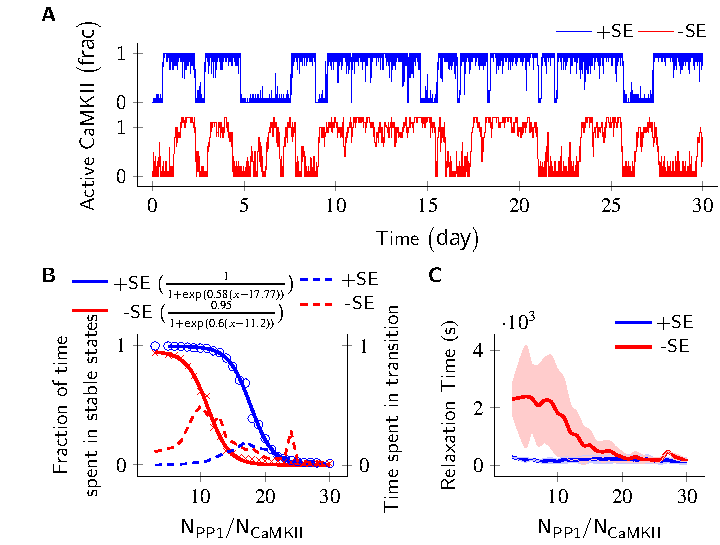
\includegraphics[width=112mm]{PaperFigures/elifeFigure2/figure_effect_of_tolerace_114mm.pdf}
    \caption{Subunit exchange improves switch tolerance of \gls{pp1}.
        \textbf{(A)} Two representative trajectories (\SUB{N}{CaMKII}=10) are
        shown with subunit exchange (+SE, blue) and without
        subunit exchange (-SE, red) respectively. \textbf{(B)} Blue and red
        solid-lines represent average activity of switch with and without 
        subunit exchange respectively. The lines are fitted with the 
        function \(\frac{a}{1+e^{k(x-x_0)}}\).
        Dotted red and blue lines show the fraction of time that the switch
        spends in intermediate states (\SUB{x}{a}\SUB{y}{n-a}, 1<a<n-1) with
        and without subunit exchange respectively. Due to subunit exchange,
        the switch tolerated a larger amount of \gls{pp1} 
        (\SUB{x}{0} value 11.2 vs 17.77 i.e., a change of 6.57 $\times$ 
        \SUB{N}{CaMKII}). Note that the range 
        of \gls{pp1} for which switch remains bistable is roughly the 
        same (k, 0.6 v/s 0.58). The fraction of time in intermediate states (dotted lines)
	is much smaller when subunit exchange is enabled (blue dotted line),
        i.e., the switching time is shorter. \textbf{(C)} Due to subunit exchange, relaxation 
        time becomes constant and independent of \SUB{N}{PP1} (blue vs red). 
        Shaded area represents standard deviation.
    }\label{fig:tolerance_pp1}
    \figdata{Source and data is available at
    \url{http://github.com/dilawar/SinghAndBhalla_CaMKII_SubunitExchange_2018/tree/master/PaperFigures/elifeFigure2}}
\end{figure}
% \end{wrapfigure}

    
We first analyzed switch sensitivity to \gls{pp1}. In our model as well in the
\gls{mz} model, the number of PP1 molecules (\SUB{N}{PP1}) had an upper
limit for the switch to exhibit bistability. This constraint arises because
\gls{pp1} must saturate in the \texttt{ON} state of the switch, i.e., 
the maximal enzymatic turnover of \gls{pp1} must be smaller than the rate of activation 
of \gls{camkii} subunits.  However, unlike the \gls{mz} model where the 
addition of one extra \gls{pp1} molecule changed the spontaneous state 
switching time (residence time) of \texttt{ON} state by roughly 90\% (Figure~2C
in \citep{miller_stability_2005}), we did not find lifetime of \texttt{ON} and
\texttt{OFF} states to be very sensitive to \gls{pp1}. In our model, it required
on average 0.5$\times$\SUB{N}{CaMKII} extra \gls{pp1} molecules to cause a 90\% 
change in the residence time. The additional number of \gls{pp1} required for 
switching is roughly equal to number of \gls{camkii} subunits in our model.

We found that the system consisting of \SUB{N}{CaMKII} holoenzymes remained
bistable for \SUB{N}{PP1}=8$\times$ to 15$\times$\SUB{N}{CaMKII} without subunit
exchange, and for \SUB{N}{PP1}=12$\times$ to 21$\times$\SUB{N}{CaMKII} with
subunit exchange. Thus, subunit exchange shifted the bistable range to higher
values of \gls{pp1}. Nevertheless, the ratio range in both cases was about the
same (blue and red sigmoidal fit in \FIG{tolerance_pp1}B).

Subunit exchange also had a strong effect on time spent by the switch in
transition from one stable state to another (relaxation time). When subunit
exchange was enabled, the relaxation time was reduced (red v/s blue dotted line
in \FIG{tolerance_pp1}B) and also became independent of \SUB{N}{PP1}.
Moreover, the standard deviation of the relaxation time was greatly reduced in
the presence of subunit exchange (red and blue curve,
\FIG{tolerance_pp1}C).

Parallel results were obtained for the effect of subunit exchange on
\gls{camkii} switch robustness in the context of protein turnover. Without
subunit exchange, switch stability as measured by residence time of the \texttt{ON}
state decreased exponentially with increasing turnover rate. With
subunit exchange, however, residence time of \texttt{ON} state remained roughly
constant upto a $\sim$10 fold increase in turnover (\FIG{turnover}B),
after which subunit exchange could not phosphorylate all inactive holoenzymes
produced by turnover, and the switch started to show exponential decay of 
stability. As expected, turnover increased the number of switching events 
in the regime of bistability in both cases.

\begin{figure}[t]
    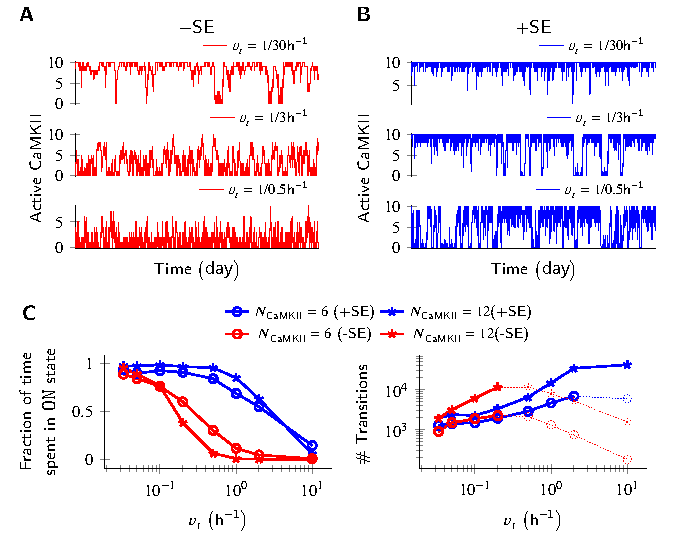
\includegraphics[width=114mm]{./PaperFigures/elifeFigure3/figure_turnover_tolerance_114.pdf}
    \caption{Subunit exchange improves switch tolerance of higher rates of
        protein turnover.
        \textbf{(A,B)} Three sample trajectories are shown for a switch of 
        size \SUB{N}{CaMKII}=10 without subunit exchange
        (-SE,red) and with it (+SE,blue). We consider three different 
        turnover rates of 1 per \SI{30}{\hour}, 1 per \SI{3}{\hour}, 
        and 1 per 0.5 \si{\hour}. As turnover is increased, the state stability 
        of the \texttt{ON} state of the switch decreases.
        \textbf{(C, left)} Normalized residence time of \texttt{ON} state vs. turnover
        rate for two switches of size 6 and 12. Without subunit exchange, switch
        stability decreases exponentially with turnover rate (red), however when
        subunit exchange is enabled, switch stability is not affected by
        turnover rates as high as \SI{1}{\per \hour} (blue). \textbf{(C,right)} In
        the bistable regime (solid lines), the number of switching events increases roughly
        linearly with turnover rate.
    }\label{fig:turnover}
    \figdata{Source and data is available at
    \url{http://github.com/dilawar/SinghAndBhalla_CaMKII_SubunitExchange_2018/tree/master/PaperFigures/elifeFigure3}}
\end{figure}

Thus, subunit exchange increases the range of \SUB{N}{PP1} and turnover rate 
over which the switch remains bistable. 

\subsection{Subunit exchange facilitates the spread of \gls{camkii}
activity}\label{res:spread_activity}

As suggested in \citep{stratton_activation-triggered_2014}, we found that
subunit exchange facilitates spread of \gls{camkii} activation
(\FIG{subunit_facilitates_spread}). When subunits were allowed to
diffuse, they could be picked by neighbouring inactive \gls{camkii} holoenzymes.
This effectively overcame the first slow step of \gls{camkii} phosphorylation
(\EQ{phospho}) thereby facilitating the spread of activation.

We put \SUB{N}{CaMKII}=18 inactive holoenzymes in a cylinder with the volume of
\SI{0.0275}{\cubic\micro\meter} and the length of \SI{540}{\nano\meter}
representing the \gls{psd}. The cylinder was divided into 18 voxels (1
holoenzyme in each voxel).  Each voxel was separated by \SI{30}{\nano\meter},
which is the average nearest-neighbour distance for \gls{camkii} holoenzymes
\citep{feng_quantitative_2011}.  Each voxel was considered to be a
\emph{well-mixed} environment i.e., diffusion was instantaneous within the
voxel. Diffusion was implemented as cross-voxel ``jump'' reactions (See
\nameref{sec:materials_and_methods}).  We did not try 2D/3D diffusion because of
its simulation complexity and because it would be expected to be qualitatively
similar \citep{fange_stochastic_2010}.

We fixed the diffusion coefficient of \gls{pp1} (\SUB{D}{PP1}) and quantified
the effect of varying the diffusion coefficient of subunits (\SUB{D}{sub}) and
basal calcium levels. We used
\SUB{D}{PP1}=\SI{0.5}{\micro\meter\squared\per\second} which is the observed
value of the diffusion coefficient of Ras, which is a similar sized protein
\citep{harvey_spread_2008}. We ran simulations for 4 hours at basal calcium
concentration [\gls{ca}]=\SI{80}{\nano M} and without subunit exchange (i.e.,
\SUB{D}{sub}=0). Here the system showed no significant \gls{camkii} activity.
When we enabled subunit exchange by setting
\SUB{D}{sub}=\SI{0.1}{\micro\meter\squared\per\second},
\FIG{subunit_facilitates_spread}B), \gls{camkii} activity rose to
maximum within \SI{4}{\hour}. As expected, the effect of subunit exchange (rise
time quantified as the time taken by \gls{camkii} to rise from 10\% to 90\%) was
stronger when the basal \gls{ca} was higher
(\FIG{subunit_facilitates_spread}C). Increasing \SUB{D}{sub} decreased
the rise time of \gls{camkii} activity.

Subunit exchange did not have any impact on the average \gls{camkii} activity at
longer time scales (\FIG{subunit_facilitates_spread}E) though we found
that long-time average \gls{camkii} activity increased when subunit exchange was
enabled. This change was independent of \SUB{D}{sub} (not due to subunit
exchange) but was strongly dependent on \SUB{D}{PP1}. This is because
potency of \gls{pp1} reduced with increased \SUB{D}{PP1}
(\FIGSUPP[subunit_facilitates_spread]{diffusion_reduces_pp1_potency}) which led to decreased \gls{pp1}
activity and hence \gls{camkii} activity.

Thus, subunit exchange facilitates the spread of kinase activity at short time
scale but does not influence its long time activity.

% \begin{SCfigure*}[\sidecaptionrelwidth][]
\begin{figure}
    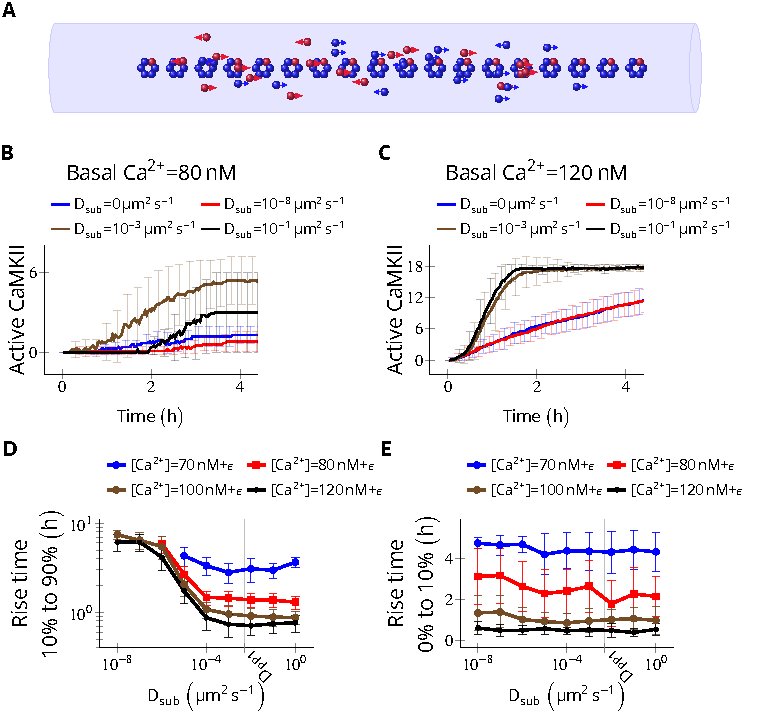
\includegraphics[width=0.95\linewidth]{./PaperFigures/elifeFigure4/figure_camkii_activation_130mm.pdf}
    \caption{Subunit exchange facilitates the spread of kinase activity
        \citep{stratton_activation-triggered_2014} but does not change its
        long-time average. \textbf{(A)} 18 CaMKII holoenzymes were put in a
        cylinder of volume \SI{0.0275}{\cubic\micro\meter} discretized into 18
        voxels, each separated by \SI{30}{\nano\meter}. For all simulations
        \SUB{D}{PP1}= \SI{0.5}{\micro\meter\squared\per\second}. \textbf{(B)}
        Activation profile of \gls{camkii} at mean basal calcium level of
        \SI{80}{\nano M} (\FIG{validation}C) for different values of
        \SUB{D}{sub}. When subunits diffused
        with zero or negligible coefficient (\SUB{D}{sub}=0 and
        \SUB{D}{sub}=\SI{e-8}{\micro\meter\squared\per\second}), mean activity
        of \gls{camkii} remained roughly zero. For \SUB{D}{sub}=\SI{0.001} and
        \SI{0.1}{\micro\meter\squared\per\second}, the mean \gls{camkii}
        activity reached its maximum within \SI{4}{\hour}.  \textbf{(C)}
        \gls{camkii} activates faster at higher mean basal calcium level of
        \SI{100}{\nano M}. \textbf{(D)} The time taken by \gls{camkii} to rise
        from 10\% to 90\% of its maximum value (rise time) in hours
        v/s \SUB{D}{sub} for different mean basal calcium levels. The effect of
        subunit exchange is more prominent at higher calcium levels for all
        values of \SUB{D}{sub}, and stronger (decreasing rise
        time) for larger \SUB{D}{sub} for all values of \gls{ca} level. 40
        trajectories were generated for each trace. Error bars represents
        standard deviation. \textbf{(E)} The onset of activity time (in hours) v/s
        \SUB{D}{sub}, where onset of activity time is measured as the time taken 
        by inactive \gls{camkii} to rise from zero to 10\% of its maximum 
        value. Average onset of activity time decreased with increasing
        basal \gls{ca} level but remained independent of \SUB{D}{sub}. Error bar
        represents standard deviation.
        \textbf{(F)} Long-time average \gls{camkii} activity (\SUB{N}{CaMKII}=6)
        is independent of \SUB{D}{sub}, and only depends on \SUB{D}{PP1}. Black
        dots represent bistable configurations with at least 4 transitions
        observed in 10 days long simulation.
    }
    \label{fig:subunit_facilitates_spread}
    \figsupp[Sample trajectories of \gls{camkii} activation for basal
    \gls{ca} concentration of \SI{100}{\nano M}.]{In all simulations,
        \SUB{D}{PP1} is fixed to \SI{e-13}{\micro\meter\squared\per\second} and \SUB{D}{sub} was
        varied. Each plot contains 40 trajectories. Dark black trajectory in
        each plot shows the average of all 40 trajectories. 
    }{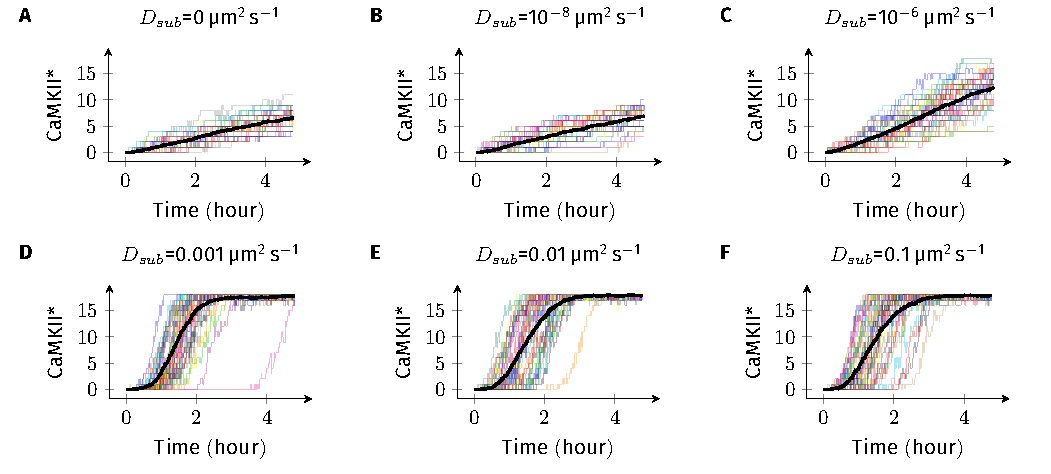
\includegraphics[width=\linewidth]{./PaperFigures/suppl/figure_camkii_activations_trajs.pdf}}
    \label{figsupp:camkii_activation_se_trajs}
    \figsupp[\gls{pp1} potency reduces as \SUB{D}{PP1} increases.]{CaMKII/PP1 system
        was put into a cylinder discretized into 6 voxels of equal volume
        separated by distance \(h\)=\SI{30}{\nano\meter}. 
        \textbf{(A)} \textbf{(above)} For each voxel, trajectory of active \gls{pp1} v/s time
        is plotted in blue. \textbf{(below)} Cross-correlation matrix (Pearson
        product-moment correlation coefficient, using \texttt{numpy.corrcoef}
        function). \textbf{(B,C)} Same as \textbf{A} but with different value of
        \SUB{D}{PP1}, \SI{0.001}{\micro\meter\squared\per\second} and
        \SI{0.1}{\micro\meter\squared\per\second} respectively. \gls{pp1} activity
        reduces in all voxels with increased \SUB{D}{PP1}. The correlation of
        \gls{pp1} activity among voxels does not improve with increased
        \SUB{D}{PP1} therefore non-linear distribution of \gls{pp1} in voxels is
        unlikely to be a significant contributor to the observed loss of \gls{pp1}
        potency. \textbf{(D)} \gls{pp1} activity decreased
        with increased \SUB{D}{PP1} but remained independent of diffusion
        coefficient of subunit (\SUB{D}{sub}). On y-axis, \gls{pp1} activity is measured as ratio
        of sum of number of all active \gls{pp1} in all voxels during the
        simulation divided by the simulation time in hours. On top, dotted blue
        line (labeled \textcolor{blue}{\SUB{D}{PP1}=0}) represents the case where
        \gls{pp1} was not allowed to diffuse. At bottom, dotted blue line
        (labeled \textcolor{blue}{1-voxel}) shows the case where the cylinder
        consists only of 1 voxel and diffusion is instantaneous i.e., it is a
        well-mixed system. As expected, as \SUB{D}{PP1} increased, the 6 voxels system converged to a
        well-mixed system of 1 voxel of 6x volume.
        Note that a similar effect is seen for a range of \SUB{D}{sub},
        including \SUB{D}{sub}=\SI{5}{\micro\meter\squared\per\second}, for
        which $h_{crit}=\SI{0.33}{\nano\meter}$, satisfying the condition \(h\gg h_{crit}\)
        \citep{isaacson_reaction-diffusion_2009}\citep{erban_stochastic_2009}.
        (Also see Fig. \FIG{suppl_reac_rdme} and \nameref{sec:diff_as_gillespie})
        Thus we do not expect that this is a numerical artifact due to our use
        of cross-voxel jump reactions to approximate diffusion. 
}{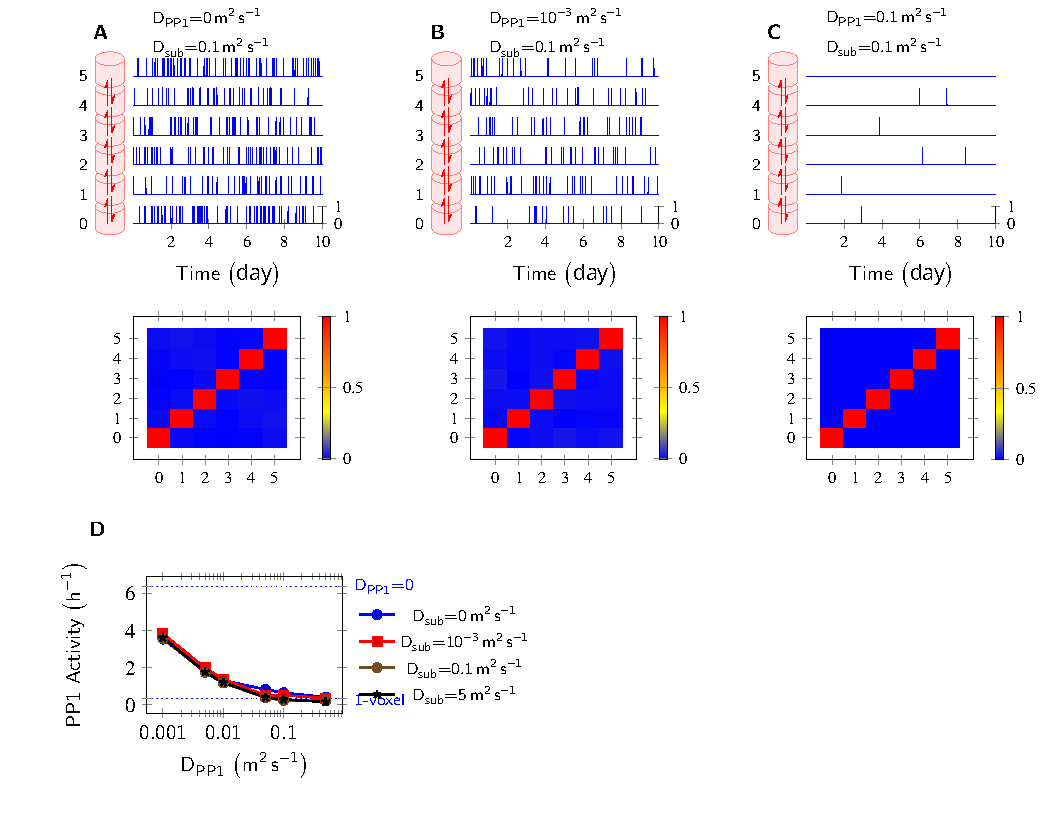
\includegraphics[width=\linewidth]{./PaperFigures/suppl/figure_pp1_profile.pdf}}
\label{figsupp:diffusion_reduces_pp1_potency}
\figdata{Source and data is available at
\url{http://github.com/dilawar/SinghAndBhalla_CaMKII_SubunitExchange_2018/tree/master/PaperFigures/elifeFigure4}}
\end{figure}


%%%%%%%%%%%%%%%%%%%%%%%%%%%%%%%%%%%%%%%%%%%%%%%%%%%%%%%%%%%%%%%%%%%%%%%%%%%%%%%
% Spread of activity and synchronization

\subsection{Subunit exchange synchronizes switching activity of clustered \gls{camkii}}\label{subsec:se_sync_switches}

\begin{figure}%[t]%[bth] 
    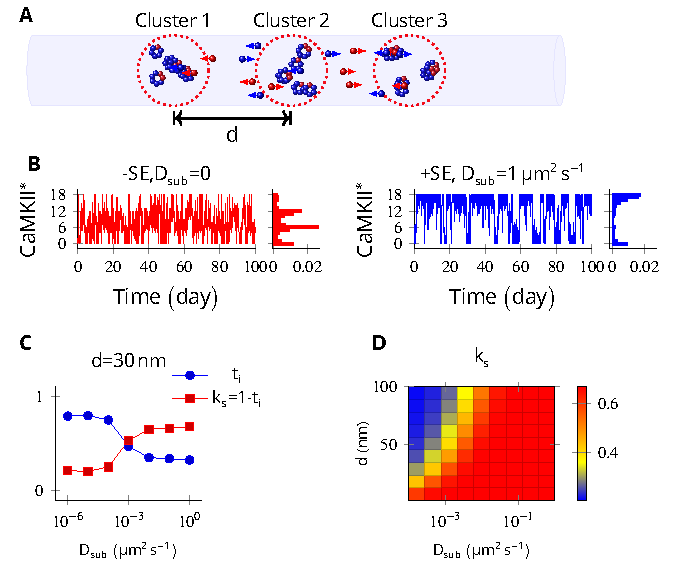
\includegraphics[width=114mm]{./PaperFigures/elifeFigure5/figure_sync_114mm.pdf}
    \caption{In \gls{psd}, subunit exchange synchronizes activity of
        \gls{camkii} clusters. \textbf{(A)} 3 clusters of
        N\textsubscript{CaMKII}=6 in \gls{psd} separated by distance \(d\).
        \gls{camkii} subunits are shown as red (inactive) and blue (active)
        balls.  Subunits and \gls{pp1} (not shown) were allowed to diffuse along
        the axis. \textbf{(B)} Without subunit exchange, all three switches
        flipped independently i.e., state distribution on right is binomial when bin size is \SUB{N}{CaMKII}
        (left, red). With subunit exchange, all switches synchronized their activity
        i.e., population acted as a single bistable switch (right, blue).  \textbf{(C)}
        Strength of synchronization (k\textsubscript{s}) v/s diffusion
        coefficient \SUB{D}{sub} for a system of 3 switches separated from each
        other by a distance \SI{30}{\nano \meter}.
        $k_s=1-t_i$ where $t_i$ is fraction of time
        spent by switches in intermediate states
        x\textsubscript{a}y\textsubscript{n-a}; 1\textless{}a\textless{}n.
        Synchronization is strong for k\textsubscript{s} \textgreater{} 0.4.
        \textbf{(D)} Phase plot of \SUB{k}{s} v/s \SUB{D}{sub} and d. The effect
        of synchronization \SUB{k}{s} due to subunit exchange is strong and
        robust to changes in \SUB{D}{sub}, and strong for $d$ as large as
        \SI{100}{\nano\meter}. \SUB{D}{PP1}=\SI{0.5}{\micro\meter\squared\per\second}
        for all simulations. 
    }\label{fig:sync_spread}
\figdata{Source and data is available at
\url{http://github.com/dilawar/SinghAndBhalla_CaMKII_SubunitExchange_2018/tree/master/PaperFigures/elifeFigure5}}
\end{figure}

Next we probed the effect of subunit exchange between spatially separated
\gls{camkii} clusters at longer timescales. We considered \SUB{N}{CaMKII}
organized into three clusters of \SUB{N}{CaMKII}/3 holoenzymes, each separated
by a distance \(d\). This configuration corresponds to cases where receptors and
\gls{camkii} holoenzymes are clustered at the synapse. 

When there is no subunit exchange across voxels i.e., \SUB{D}{sub}=0, these
switches are expected to switch independently like multiple coins flipped
together, resulting in a binomial distribution of activity. The clustered system
had 3 relatively stable bistable systems (long residence time,
\FIG{validation}E). As expected, without subunit exchange, activity in
this system had a binomial distribution (\FIG{sync_spread}B, red plot). 

Then we allowed \gls{pp1} and \gls{camkii} subunits to undergo linear diffusion.
We fixed \SUB{D}{PP1}=\SI{0.5}{\micro\meter\squared\per\second} as before and varied
$\SUB{D}{sub}$ to quantify effect of subunit exchange.  Subunit exchange led to
synchronization of switching activity. The population of clustered \gls{camkii}
acted as a single bistable switch (\FIG{sync_spread}B, blue plot).
This effect was strong and robust to variation in \SUB{D}{sub}. Even for a very
small value of \SUB{D}{sub}=\SI{0.01}{\micro\meter\squared\per\second}, we observed
strong synchronization (\FIG{sync_spread}D). The synchronization
disappeared completely for diffusion coefficient less than
\SUB{D}{sub}=\SI{e-4}{\micro\meter\squared\per\second} for distance
\SI{30}{\nano\meter} (\FIG{sync_spread}D).

Thus, for most physiologically plausible values of diffusion coefficient
\SUB{D}{sub}, subunit exchange causes synchronization of switching activity of
clustered \gls{camkii}.

\subsection{Subunit exchange may account for the observed dual decay rate of
\gls{camkii} phosphorylation}\label{subsec:camkii_decay_two_time_course}

Finally, we asked if subunit exchange might account for the complex time-course
of \gls{camkii} dynamics in spine as observed in recent experiments
\citep{chang_camkii_2017}. We designed an experiment to replicate an experiment
where \gls{camkii} was inhibited by a genetically encoded photoactivable
inhibitory peptide after activating it by glutamate uncaging
\citep{murakoshi_kinetics_2017}. In the spine, \gls{camkii} is more accessible to
phosphatases than in the \gls{psd}, where our previous calculations had been
located. To model the increased availability of phosphatases, we increased the
number of \gls{pp1} by an order of magnitude, and increased the volume of the
compartment to match the volume of a typical spine head i.e.,
\SI{0.02}{\cubic\micro\meter} \citep{bartol_nanoconnectomic_2015}. We found that
CaMKII acted as a integrator of calcium activity with typical exponential decay
dynamics (\FIG{cytosol_integrator}A). We then enabled the diffusion of
\gls{camkii} subunits and \gls{pp1} with same diffusion coefficient
\SUB{D}{sub}=\SUB{D}{PP1}=\SI{1}{\micro\meter\squared\per\second}.  These
conditions decreased the rate of dephosphorylation of \gls{camkii} holoenzymes
significantly. The decay dynamics could not be fitted using a simple exponential
(\FIG{cytosol_integrator}B). With our values of parameters, decay rate
decreased by an order of magnitude when subunit exchange was enabled
(\FIG{cytosol_integrator}B).

% This figure is one column.
\begin{figure}%[t]%[tbh]
    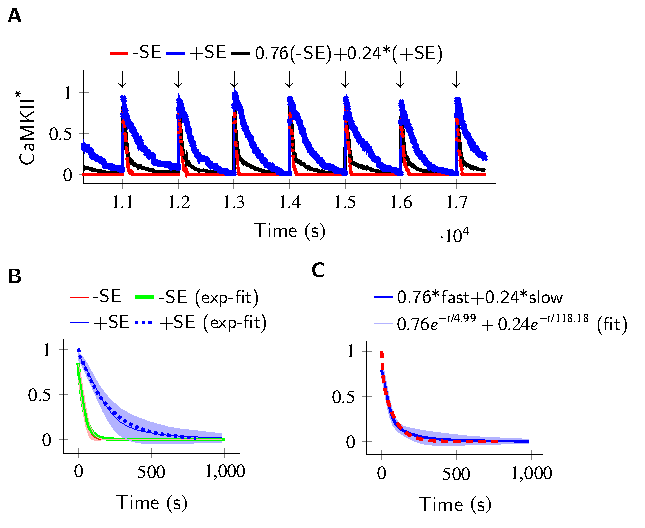
\includegraphics[width=11.4cm]{PaperFigures/elifeFigure6/figure_two_timecourses_114cm.pdf}
    \caption{ \gls{camkii} acts as a leaky integrator of \gls{ca} activity in
        spine cytosol which decays with two time-courses. The slow decaying
        integrator is formed due to clustering of \gls{camkii} in the cytosol.
        At small distance subunit exchange remains effective in the \gls{pp1} rich cytosol.
        \textbf{(A)} Trajectories of \gls{camkii} activity (fraction of total \gls{camkii})
        are shown when a strong \gls{ca} pulse of the duration of \SI{3}{\second}
        was applied to the system after every \SI{1000}{\second} ($\downarrow$).
        The \gls{ca} pulse (\SI{1e-3}{mM}) is strong enough to activate roughly
        all \gls{camkii}. After the pulse, \gls{ca} levels were brought down to basal level (Fig
        1C). Three trajectories are plotted: without subunit exchange (red), with
        subunit exchange (blue), and a weighed sum of red and blue (74\%
        red + 24\% blue as estimated in \cite{chang_camkii_2017}). 
        \textbf{(B)} Average decay dynamics for \SI{1000}{\second} after the
        onset of strong \gls{ca} pulse ($\downarrow$).  When there is no subunit exchange, 
        \gls{camkii} decays at timescale of approximately \SI{41.61}{\second}
        (dashed yellow). When subunit exchange is enabled, \gls{camkii} decay has larger
        time-constant of $\SI{200.84}{\second}$ (dashed blue). 
        \textbf{(C)} Dynamics of mixed population (black, raw data shown in
        black in \textbf{A}). Fit of mixed population by a double
        exponential for known weights (74\% fast + 26\% slow) (dashed red).
        Time constants are estimated to be \SI{8.39}{\second} for fast and
        \SI{86.2}{\second} for slow population by the fit. Double exponential plotted
        with parameters estimated in \cite{chang_camkii_2017} (magenta) i.e
        $0.74e^{-t/6.4}+0.26e^{-t/92.6}$ (only mean is shown). Experimental data
        matches well with double exponential fit (magenta v/s dashed red).
        Shaded areas are the standard deviation. All fits were performed using
        gnuplot (version 5.2.4).
    }\label{fig:cytosol_integrator}
\figdata{Source and data is available at
\url{http://github.com/dilawar/SinghAndBhalla_CaMKII_SubunitExchange_2018/tree/master/PaperFigures/elifeFigure6}}
\end{figure}

We expected subunit exchange to have a strong effect on the decay activity of 
clustered \gls{camkii} in spine cytosol (e.g., \gls{camkii} bound to actin)
because of the proximity of holoenzymes, leading to rapid exchange. 
Our simulations supported this prediction. If there are populations of 
clustered as well as non-clustered \gls{camkii} in the spine, we expect that
they will exhibit long and short time-courses of activity decay.

Thus, we suggest that subunit exchange may be a mechanism that leads to
\gls{camkii}$\alpha$ activity decaying with two time-courses in spine 
cytosol \citep{chang_camkii_2017}.


% DISCUSSION
\section{Discussion}\label{discussion}

Here we have shown that subunit exchange strongly affects the properties of
CaMKII/PP1 pathway, both in its role as a bistable switch in PSD and as an
integrator of \gls{ca} activity in spine cytosol. In the PSD, where the model was
tuned to elicit bistable dynamics from clustered \gls{camkii}, subunit exchange
improved the stability of \gls{camkii}/\gls{pp1} switch by synchronizing the
kinase activity across PSD (\FIG{cytosol_integrator}). It also improved
\gls{camkii} tolerance of PP1 and turnover rate (\FIG{tolerance_pp1}
and \FIG{turnover}). In the case where \gls{camkii} was uniformly
distributed in \gls{psd}, subunit exchange facilitated more rapid activation of
\gls{camkii} (\FIG{subunit_facilitates_spread}BCD) 
\citep{stratton_activation-triggered_2014}.  These simulation results predict
that a \gls{camkii} mutant lacking subunit exchange would be deficient in 
switch stability and slower to activate.

In the spine head, subunit exchange facilitated integration by prolonging the
decay time-course of kinase activity (\FIG{cytosol_integrator}).  The
fact that \gls{camkii} dynamics changed from an integrator to bistable switch as
we moved from spine cytosol (a phosphatase rich environment) to the \gls{psd}
(where PP1 is tightly controlled) suggests an interesting
sub-compartmentalization of functions in these microdomains. Furthermore, we
observed that the clustering of \gls{camkii} had important implications for its
sustained activity.

\Gls{camkii} is non uniformly distributed in \gls{psd} where it is mostly
concentrated in a small region of \SI{16}{\nano \meter} to \SI{36}{\nano \meter}
below synaptic cleft \citep{petersen_distribution_2003}. In \gls{psd}, \gls{camkii} may exist in
large clusters given that \gls{psd} is rich in \gls{camkii} binding partners.
Our study predicts that subunit exchange may lead to synchronization when
\gls{camkii} is clustered, or more rapid activation by calcium when it is uniformly
distributed. Given that \gls{camkii} can form clusters with \gls{nmda}
receptors, it would be interesting to study the mixed case where some
\gls{camkii} is clustered and rest is uniformly distributed. This would require
detailed 3D simulation and is beyond the scope of this study.

Subunit exchange is unlikely to have any impact on neighbouring spines. The mean
escape time of a single \gls{camkii} subunit from a typical spine is between
\SI{8}{\second} to \SI{33}{\second} \citep{holcman_diffusion_2011}. In a real
synapse, this time would be even larger given that \gls{camkii} interacts with
many other molecules. Any phosphorylated subunit is almost certain to be
de-phosphorylated by \gls{pp1} during this time. We therefore predict that the
effects of synchronization are local to each \gls{psd}, where \gls{pp1} is known
to be tightly controlled.  Subunit exchange loses its potency in the phosphatase
rich region of the bulk spine head or dendrite. We therefore consider it
unlikely that \gls{camkii} subunit exchange plays any role in intra-spine
information exchange such as synaptic tagging.

Finally, we suggest that existence of diverse time-scales of \gls{camkii}
activity in the PSD and spine head has important theoretical implications. A
very plastic synapse is good at registering activity dependent changes
(learning) but bad at retaining old memories. On the other hand, a rigid synapse
is good at retaining old memories but is not efficient for learning. A
theoretical meta-model which sought to strike a balance between these two
competing demands requires that diversity of timescales should exist at the
synapse \citep{benna_computational_2016}. In this model, complex synapses with
state variables with diverse time-scales are shown to form a memory network in
which storage capacity scales linearly with number of synapses, and memory decay
follows \(1/\sqrt{t}\) --- a power-law supported by psychological studies
\citep{wixted_form_1991}. This model requires memory trace to be first stored in
a fast variable and then progressively and efficiently transferred to slower
variables.  Our study suggests a concrete mechanism for such a process. Here,
calcium concentration in PSD can be mapped to the fastest variable.  The
\gls{camkii} integrator in cytosol could represent the second slower variable to
which the trace is transferred from calcium. Further, the state information is
transferred to the third slower \gls{camkii} bistable switch. The dynamics of
\gls{camkii} in the PSD forms an even slower bistable variable for longer
retention of the memory trace. It is possible that memory is transferred from
here to even slower variables, such as sustained receptor insertion
\citep{hayer_molecular_2005}, PKM-$\zeta$ activation \citep{sacktor_memory_2012},
or local protein synthesis \citep{aslam_translational_2009}.

% MATERIALS AND METHODS
\section{Methods and Materials}{\label{sec:materials_and_methods} 
We extended Miller and Zhabotinksy (MZ model) \citep{miller_stability_2005}
to incorporate \emph{subunit exchange} and diffusion. We treat the
\gls{camkii} ring as proxy for the holoenzyme because vertical dimers are
inserted or released together \citep{bhattacharyya_molecular_2016}. We assume
that both subunits of a vertical dimer phosphorylate and de-phosphorylate
together. 

In our model, a \gls{camkii} ring with $n$ subunits ($n$=6 or 7) can exist
in 15 different states enumerated as $x_{a}y_{n-a}$ for $0 \le a \le n$ where
$x$ and $y$ represents un-phosphorylated and phosphorylated subunits
respectively. We ignore all rotational permutations and kinetically unlikely
cases where there are discontiguous phosphorylated subunits in the ring. We
assumed that the phosphorylation of neighbouring subunit proceeds clockwise.


\subsection{Phosphorylation and dephosphorylation of \gls{camkii} ring}\label{phosphorylation-and-dephosphorylation-of-ring} 

The activation of \gls{camkii} follows the same dynamics as in \gls{mz} model
(\EQ{phospho}).  The first step in \gls{camkii} activation requires
simultaneous binding of two \gls{cacam} to the two adjacent subunits of
\gls{camkii}. Once a subunit is phosphorylated, it catalyzes phosphorylation of
it's neighbour (\emph{auto-phosphorylation}) which requires binding of only one
\gls{cacam}. Therefore, further phosphorylation proceeds at much faster rate.
Once fully phosphorylated, \gls{camkii} moves to \gls{psd} where it binds to
\gls{nmda} receptor. Upon binding, it is no longer accessible other phosphatases
save \gls{pp1}.

\begin{equation}\label{eq:phospho}
    \newcommand\CaHILL{\ensuremath{\frac{Ca^{2+}}{K_{H1}}}}
    \newcommand\VONE{k_1 \left[\frac{H^3}{1+H^3}\right]^2}
    \newcommand\VTWO{k_1\frac{H^3}{1+H ^3}}
\begin{gathered}
    x_ay_{n-a} \xrightarrow{v_1} x_{a-1}y_{n-a+1} \xrightarrow{v_2} x_{a-2}y_{n-a+2} \\
    H=\CaHILL,\, v_1 = \VONE,\, v_2 =\VTWO
\end{gathered}
\end{equation} where $n=6\;\text{or}\;7$, and $1\le a \le n$.

The dephosphorylation of the \gls{camkii} ring, and the subunit follow a
Michaelis-Menten like scheme \EQ{dephosphorylation}. We implemented this 
as coupled mass-action chemical reactions.
\begin{equation}\label{eq:dephosphorylation}
    \begin{gathered}
        PP1 + x_ay_{n-a} \xrightleftharpoons[k^-]{k^+} PP1.x_ay_{n-a} 
            \xrightarrow{k_2} PP1 + x_{a+1}y_{n-a-1} \\
        PP1 + x \xrightleftharpoons[k^-]{k^+} PP1.x \xrightarrow{k_2} PP1 + y
    \end{gathered}
\end{equation} where $n=6\;\text{or}\;7$, and $1\le a \le n$. Following Miller
et al. \citep{miller_stability_2005}, we assumed $k^-=0$. This gave us
$k^+=\frac{k_2}{k_M}=\SI{1}{\per\micro M\per\second}$.

\subsection{Subunit exchange}\label{subunit exchange}
Since \gls{camkii} ring consists of either 6 or 7 subunits exists in our model,
any ring with 6 subunits cannot lose a subunit, and a ring with 7 subunits cannot
gain a subunit. The reactions which result in either gain or lose of a
subunit are given by \EQ{losegainx} where $0\le a \le 6\text{ or }7$.
%\begin{equation}\label{eq:losegainx}
%    \begin{gathered}
%    x_ay_{7-a} + x \xrightleftharpoons[k^-_x]{k^+_x} x_{a+1}y_{6-a},\,0\le a\le 7 \\
%    x_ay_{6-a} + y \xrightleftharpoons[k^-_y]{k^+_y} x_{a}y_{7-a},\,0\le a \le 6
%    \end{gathered}
%\end{equation}
\begin{equation}\label{eq:losegainx}
    \begin{gathered}
    x_ay_{7-a} + x \xrightleftharpoons[k^-_x]{k^+_x} x_{a+1}y_{6-a},\,
    x_ay_{6-a} + y \xrightleftharpoons[k^-_y]{k^+_y} x_{a}y_{7-a}
    \end{gathered}
\end{equation}
The values of $k_x^+$, $k_x^-$, $k_y^+$, and $k_y^-$ are not available in the
literature that we are aware of. Bhattacharya \textit{et al}. 
\citep{bhattacharyya_molecular_2016} speculate that upon activation, the hub
of holoenzyme becomes less stable and more likely to open up and lose a subunit
i.e., active holoenzymes may lose subunits faster. Therefore, we maintained the
following ratio \(k_x^- = 10 k_x^+ N_{\text{CaMKII}}\) and \(k_y^- = 10 k_y^+
N_{\text{CaMKII}}\) in all simulations.

\subsection{\gls{pp1} deactivation}\label{subsec:pp1_deactivation} 
In the \gls{psd}, \gls{pp1} is the primary -- and perhaps only -- phosphatase known to
dephosphorylate \gls{camkii}\citep{strack_translocation_1997}.  We followed
\gls{mz} model for \EQ{i1pandpp1} where $I1$ is \gls{i1} which inactivates
\gls{pp1} (See SI for more details). \Gls{i1p} renders \gls{pp1} inactive by
forming \gls{i1ppp1}. 
\begin{equation}\label{eq:i1pandpp1}
    \begin{gathered}
        \text{PP1} + \text{I1P} \xrightleftharpoons[k_4]{k_3} \text{I1P.PP1} \\
        \text{I1P} = \text{I1} \frac{v_{PKA}}{v_{CaN}} 
            \frac{1+\left(\frac{Ca}{k_{H2}}\right)^3}{\left(\frac{Ca}{k_{H2}}\right)^3}
    \end{gathered}
\end{equation}

\subsection{Turnover}\label{turnover}
The turnover of \gls{camkii} is a continuous process with rate
$v_{t}$ \si{\per\second} \EQ{turnover}.
\begin{equation} \label{eq:turnover}
    \begin{gathered}
        x_ay_{6-a} \xrightarrow{v_t} x_6y_0,\;
        x_ay_{7-a} \xrightarrow{v_t} x_7y_0,\; \text{for } a \ge 1
    \end{gathered}
\end{equation}

\subsection{\gls{ca} influx}


\subsection{Diffusion and simulation method}\label{subsec:simulator}
Diffusion is implemented as cross voxel ``jump'' reaction. Diffusion of a
species X with diffusion-coefficient \SUB{D}{X} between voxel A and B separated
by distance $h$ is modelled by reaction $X_A \xrightleftharpoons[k]{k} X_B$
where \( k={D_X}/{h^2}\), and \([X_A]=[X_B]=[X]/2 \)
\citep{erban_practical_2007}.  Based on our own numerical results (see SI) and
other studies \citep{isaacson_reaction-diffusion_2009,erban_stochastic_2009}, we
are confident that \( h \ge 10h_{crit}\) where
\(h_{crit}=\frac{k^+}{D_{PP1}+D_{sub}}\) is a good value
\citep{erban_stochastic_2009}.  We have \( h_{crit} \le \SI{3.2}{\nano\meter} \)
whenever $D_{PP1}+D_{sub}\ge\SI{0.5}{\micro\meter\squared\per\second}$. For all
simulations presented in main text, we maintain $h\ge h_{crit}$.  For a case
where $h$ is smaller than $h_{crit}$ in some trajectories see
\FIGSUPP[subunit_facilitates_spread]{diffusion_reduces_pp1_potency}. 

All simulations were performed using Stochastic solver (Gillespie method)
available in MOOSE simulator (\url{https://moose.ncbs.res.in}, version 3.1.4)
\citep{ray_pymoose:_2008}. This model is available
at \url{https://github.com/dilawar/SinghAndBhalla_CaMKII_SubunitExchange_2018}.
Table of parameters can be found in SI (\TABLE{si:parameters}).

\subsection{Table of parameters} 
\TABLE{si:parameters} summarizes parameters of our model.

\begin{singlespace}
\begin{table}[t] %[hbt]
    \caption{Table of parameters used in model.}\label{tab:si:parameters}
    \begin{tabularx}{\linewidth}{p{15mm} p{0.4\linewidth} X X}
        \toprule
        \textbf{Symbol} & \textbf{Parameter} & \textbf{Value} & \textbf{Ref}\\
        \midrule
        V\textsubscript{Spine} & Volume of Spine & 1 to \SI{5e-20}{\cubic \meter} & \citep{bartol_nanoconnectomic_2015}\\ 
        V\textsubscript{PSD} & Volume of PSD (Thickness 
                                \texttildelow\SI{100}{\nano \meter}. 
                                Surface area \texttildelow\SI{0.05}{\cubic\micro\meter}) 
                             & 1 to \SI{5e-21}{\cubic \meter} 
                             & \citep{farley_structure_2015}, \citep{bartol_nanoconnectomic_2015}\\
        N\textsubscript{CaMKII} & Total CaMKII holoenzymes in PSD/Spine & 100$\pm$18 & \citep{farley_structure_2015}\\
        N\textsubscript{PP1} & Total PP1 in PSD & 4 to 20\(\times\)N\textsubscript{CaMKII} & This paper\\
                             & Total PP1 in Spine & 10 to 100\(\times\)N\textsubscript{CaMKII} & This paper\\
        I1 & Concentration of free
        I1 & \SI{0.1}{\micro M} & \citep{miller_stability_2005}\\
        V\textsubscript{CaN} & Activity of calcineurin divided by its Michaelis
        constant & \SI{1.0}{\per \second} & \citep{miller_stability_2005}\\
        V\textsubscript{CaM} & Activity of PKA divided by its Michaelis
        constant & \SI{1.0}{\per \second} & \citep{miller_stability_2005}\\
        K\textsubscript{M} & The Michaelis constant of
        PP1 & \SI{10}{\micro M} & 0.4 to 20 \si{\micro M} \citep{zhabotinsky_bistability_2000}\\
        K\textsubscript{H1} & Hill constant of CaMKII (\gls{ca})
        activation) & \SI{0.7}{\micro M} & \citep{koninck_sensitivity_1998}\\
        n\textsubscript{H1} & Hill coefficient of CaMKII (\gls{ca})
        activation) & 3 & \citep{stemmer_dual_1994}\\
        K\textsubscript{H2} & Hill constant of calcineurin (\gls{ca}
        activation) & \SI{0.3}{\micro M} & \citep{stemmer_dual_1994}\\
        n\textsubscript{H2} & Hill constant of calcineurin
        (\gls{ca} activation) & 3 & \citep{stemmer_dual_1994}\\
        k\textsubscript{1} & The catalytic constant of
        autophosphorylation & \SI{1.5}{\per\second} & \citep{hanson_dual_1994}\\
        k\textsubscript{2} & The catalytic constant of protein
        phosphotase & \SI{10}{\per\second} & \citep{bradshaw_ultrasensitive_2003,ichikawa_interactions_1996}\\
        k\textsubscript{3} & The association rate constant of PP1.I1P
        complex & \SI{100}{\micro M^{-1}\second^{-1}} &
        \citep{endo_multiple_1996,miller_stability_2005}\\
        k\textsubscript{4} & The dissociation rate constant of PP1.I1P
        complex & \SI{0.1}{\second^{-1}} & \citep{endo_multiple_1996,miller_stability_2005}\\
        k\textsubscript{x}\textsuperscript{+} & The rate of adding 
        unphosphorylated subunit x & \SI{0.1}{\per\second\per \SUB{N}{CaMKII}} & This paper\\
        k\textsubscript{y}\textsuperscript{+} & The rate of adding
        phosphorylated subunit y & \SI{0.1}{\per\second\per\SUB{N}{CaMKII}} & This paper\\
        k\textsubscript{x}\textsuperscript{-} & The rate of losing
        unphosphorylated subunit x & \SI{1}{\per \second} & This paper\\
        k\textsubscript{y}\textsuperscript{-} & The rate of losing
        phosphorylated subunit y & \SI{1}{\per \second} & This paper\\
        v\textsubscript{t} & Turnover rate of CaMKII & \SI{30}{\hour^{-1}} &
        \citep{ehlers_activity_2003,miller_stability_2005}\\
        D\textsubscript{PP1} & Diffusion coefficient of \gls{pp1} & 
        \SI{0.5}{\micro\meter\squared\per\second} & This paper and
        \citep{harvey_spread_2008}\\
        D\textsubscript{sub} & Diffusion coefficient of \gls{camkii} subunits & 
        \SI{e-5} to \SI{10}{\micro\meter\squared\per\second} & This paper \\
        \bottomrule
    \end{tabularx}
\end{table}
\end{singlespace}


%%  ACKNOWLEDGEMENTS %%
\section{Acknowledgements}
We'd like to thank Marcus Benna, Stefano Fusi and Moitrayee Bhattacharyya for
discussions related to their work, Mukund Thattai for useful discussions on the
stochastic reaction diffusion methods, and Bhanu Priya for useful comments on
the manuscript. This work was funded by NCBS/TIFR and SERB JC Bose fellowship
\texttt{SB/S2/JCB-023/2016} to USB.

\bibliography{bibliography} 

\appendix
\begin{appendixbox}

% alternative row
\subsection*{Stochastic diffusion using cross-voxel reactions}\label{sec:diff_as_gillespie}

In our model, diffusion of any molecule is linear i.e., the molecules diffuse
along the axis of cylinder. The cylindrical compartment of length $L$ and radius $r$
is divided into $n$ \emph{well-mixed} voxels of length $h$ ($h=L/n$) i.e., within
a voxel, diffusion is instantaneous.  

Diffusion is implemented as cross-voxel reactions in which a molecule
\emph{jump} to its neighbouring voxels with a rate constant $k$ which is a
function of diffusion coefficient $D$ and length of voxel $h$. For example,
assume that molecule A with diffusion coefficient of $D_A$ is put into a
cylinder. We divide the entire cylinderical volume into $n$ voxels. We uniformly
distribute all molecules of A into these $n$ voxels. Any molecule from voxel $i$
(labelled $A_i$) can only jump to neighbouring voxel $i+1$ or $i-1$ with rate
$k_D^A$. This process is described by following chemical reactions (\EQ{stoch_diff}).

\begin{equation}
\begin{gathered}
    \ldots A_{i-1} \xrightleftharpoons[k_D^A]{k_D^A} A_{i}
    \xrightleftharpoons[k_D^A]{k_D^A} A_{i+1} \ldots
\end{gathered}
\label{eq:stoch_diff}
\end{equation}


\subsection*{Stochastic diffusion with bimolecular reaction}\label{subsec:rdme}

Consider a cylindrical arena with a bimolecular reaction $A+B \rightarrow \phi$.
Both A and B diffuses while $\phi$ does not. In our model, this reaction
resembles dephosphorylation of subunit or \gls{camkii} holoenzyme by \gls{pp1} .
If we divide the cylinder into $n$ voxels labelled 1, 2, $\ldots$, $n$, then we
have following resultant chemical system.

This system is completely described by following reactions.

\begin{equation}
    \begin{gathered}
        A_1 + B_1 \xrightarrow{k} \phi_1 \\
        A_2 + B_2 \xrightarrow{k} \phi_2 \\
        \vdots \\
        A_n + B_n \xrightarrow{k} \phi_n \\
        A_1 \xrightleftharpoons[k_D^A]{k_D^A} A_2 ,\, A_2 \xrightleftharpoons[k_D^A]{k_D^A} A_3 
            ,\, \ldots,\, A_{n-1} \xrightleftharpoons[k_D^A]{k_D^A} A_n \\ 
        B_1 \xrightleftharpoons[k_D^B]{k_D^B} B_2 ,\, 
            B_2 \xrightleftharpoons[k_D^B]{k_D^B} B_3 ,\, 
            \ldots,\, B_{n-1} \xrightleftharpoons[k_D^B]{k_D^B} B_n \\ 
    \end{gathered}
    \label{eq:discrete}
\end{equation}

\begin{center}
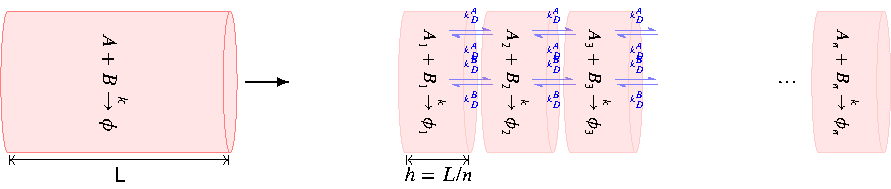
\includegraphics[width=0.8\linewidth]{./PaperFigures/suppl/figure_diff.pdf}
\captionof{figure}{Summary of the stochastic reaction diffusion method employed.}
\end{center}

Where $k_D^A=\frac{D_A}{h^2}$ and $k_D^B=\frac{D_B}{h^2}$ and
$[A_1]=[A_2]=\ldots=[A_n]=[A]$, $[B_1]=[B_2]=\ldots=[B_n]=[B]$ where $[X]$ is
concentration of X.

For system described by \EQ{discrete}, as $h$ decreases, the accuracy of
method increases first after which it starts decreasing. Specifically, the
diffusion component of system become more accurate as $h$ decreases but
bimolecular reactions events starts decreasing when Gillespie method is used
\citep{gardiner_correlations_1976}. Analytical methods  suggests a lower bound on
$h$, namely $h\gg \frac{k}{D_A+D_B}$ below which the method is likely to
produce large errors \citep{isaacson_reaction-diffusion_2009}. A numerical
study \citep{erban_stochastic_2009} suggests that $h\ge 10\frac{k}{D_A+D_B}$ is
a good value to keep the errors less than 1\% in distributions.

\begin{center}
    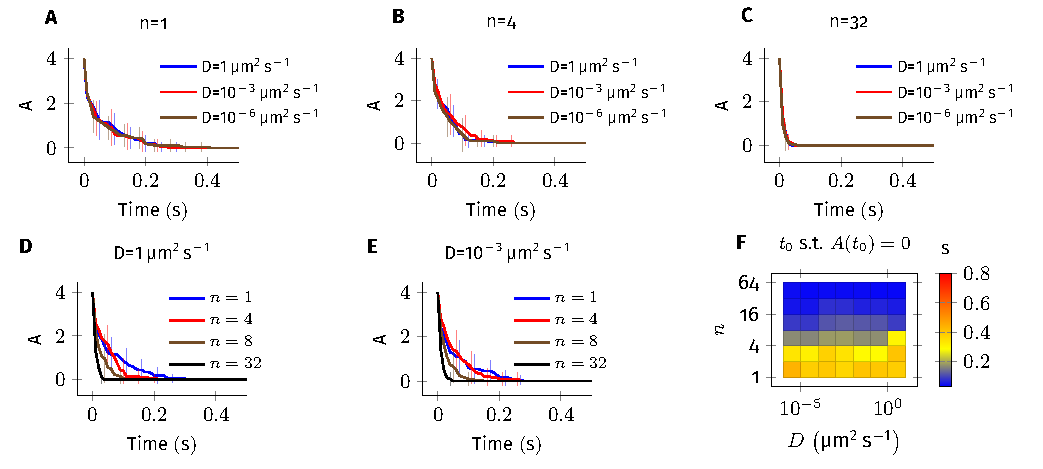
\includegraphics[width=\linewidth]{PaperFigures/suppl/figure_bimolecular_reac_rdme.pdf}\label{si:fig:discretization}
    \captionof{figure}{Error estimates for bimolecular reaction
        $A+B\xrightarrow{k} \phi$ where
        $k=\SI{1e3}{\meter\cubed\per\mole\per\second}$. Parameters of this
        system are similar to the reaction \EQ{dephosphorylation} in main text. 
        4 molecules of A and B each are put into a cylinder 
        of length $L$=\SI{500}{\nano\meter} and radius $r$=\SI{20}{\nano\meter}. This arena is divided into $n$
        equal subvolumes, each of length $h=L/n$.  Diffusion of A and B is implemented as described in eq.
        \EQ{discrete} in \nameref{subsec:rdme} where $D_A=D_B=D$.
        {\bf(A,B,C,D,E)} Average of 20 trajectories of A vs time (error bars are
        standard-deviation) for different combinations of $n$ and $D$. For fixed
        value of $n$, kinetics are undistinguishable from each other for non-zero
        value of $D$ (A, B and C). This suggests that the results described in 
        \FIGSUPP[subunit_facilitates_spread]{diffusion_reduces_pp1_potency} are majorly not due to 
        computational errors. For fixed value of $D$, however, changing $n$ has
        huge impact on dynamics of A (D,E) especially when there is less than 1 molecule in
        each voxel (compare plots where n=1,4 vs n=8,16). {\bf(F)} Time for A to reach zero
        ($t_0$) vs $D$ and $n$. 
    }
    \label{fig:suppl_reac_rdme}
\end{center}

\end{appendixbox}

\end{document}

